%! Author = quent
%! Date = 09/02/2025

\documentclass{article}
\usepackage{graphicx}
\usepackage{amsmath}
\usepackage{verbatim}  % Pour les blocs de code
\usepackage{float}     % Pour le positionnement des images
\usepackage{subcaption} % Pour afficher plusieurs images en sous-figures

\title{\textbf{Analyse des Donn\'ees - TP2}}
\author{Quentin Garnier}
\date{2025}

\begin{document}

    \maketitle

    \section{Criminalité aux USA}
    \subsection{Exploration élémentaire}
    \subsubsection{Identification des valeurs atypiques}

    Pour détecter des valeurs atypiques dans notre jeu de données, nous analysons d'abord les statistiques descriptives. En observant la variable \textbf{robbery}, nous constatons que :

    \begin{itemize}
        \item Le \textbf{3ème quartile (Q3)} est de 155.85.
        \item La valeur \textbf{maximale} est de 472.0.
    \end{itemize}

    Afin de valider cette observation, nous afficons le \textbf{boxplot} de la variable \textit{robbery}. Comme prévu, nous voyons un point isolé au-dessus de la moustache supérieure, ce qui confirme la présence d'une valeur extrême.

    Cette valeur pourrait correspondre à un état où les taux de vols avec violence sont exceptionnellement élevés. Une anlyse plus approfondie permettrait d'identifier les causes sous-jacentes de cette anomalie.

    \begin{figure}[H]
        \centering
        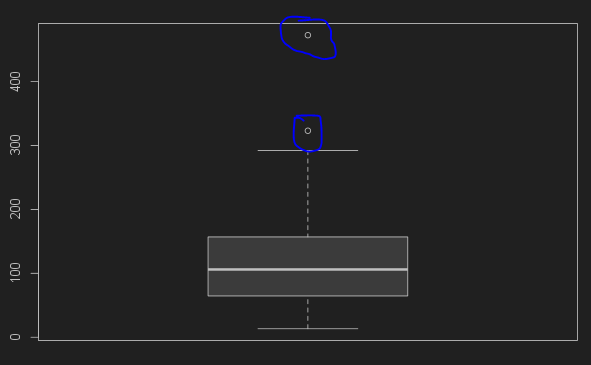
\includegraphics[width=0.5\linewidth]{img/robbery_data_boxplot}
        \caption{BoxPlot des données de robbery}
    \end{figure}

    L’analyse de la matrice de corrélation nous permet d’identifier des relations entre les différentes variables criminelles.

    \subsubsection{Corrélations fortes}
    Certaines variables montrent une corrélation élevée, indiquant une relation sgnificative :
    \begin{itemize}
        \item \textbf{Rape et Assault} : 0.74 (forte corrélaton positive)
        \item \textbf{Burglary et Larceny} : 0.79 (forte corrélation positive)
        \item \textbf{Rape et Burglary} : 0.71 (forte corrélation positivbe)
    \end{itemize}

    \subsubsection{Corrélations faibles ou inexistantes}
    Certaines variables ne montrent pas de lien significatif :
    \begin{itemize}
        \item \textbf{Murder et uto} : 0.06
    \end{itemize}

    \subsubsection{Interprétation}
    L'analyse révèle deux grands groupes :
    \begin{itemize}
        \item \textbf{Les crimes violents} (Murder, Rape, Assault, Robbery) sont fortement corrélés entre eux.
        \item \textbf{Les crimes contre les biens} (Burglary, Larceny, Auto) montrent également une forte corrélation.
        \item Il y a peu de lien entre ces deux goupes
    \end{itemize}

    \subsection{Analyse en Composantes Principales (ACP)}

    \subsubsection{Réalisation de l’ACP}
    Nous effectuons l'ACP sur la table \texttt{crime}

    \subsubsection{Choix de la dimension}

    L’analyse des corrélations montre deux groupes principaux :
    \begin{itemize}
        \item \textbf{Crimes violents} : Murder, Rape, Assault, Robbery
        \item \textbf{Crimes contre les biens} : Burglary, Larceny, Auto
    \end{itemize}

    \subsubsection{Représentation des individus et vriables}

    \subsubsection{Variance des composantes}
    Le graphique ci-dessous montre la variance expliquée par chaque composante :
    \begin{figure}[H]
        \centering
        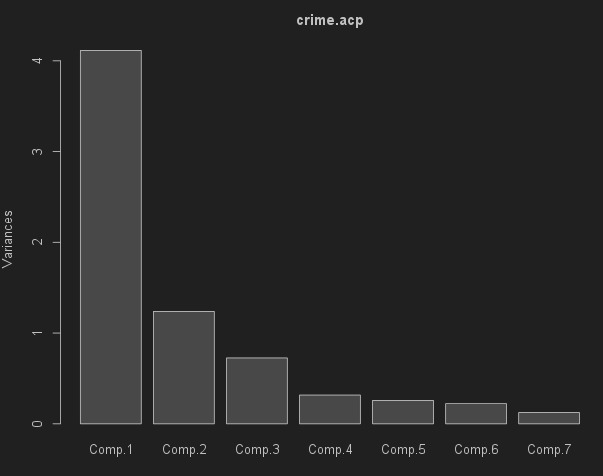
\includegraphics[width=0.5\linewidth]{img/plotcrimacp}
        \caption{BoxPlot des données de robbery}
    \end{figure}

    \textbf{Observation :} Les deux premières composantes expliquent l’essentielde la variance, les suivantes apportent peu d’information.

    \subsubsection{Confirmation du choix de la dimension}
    Les biplots permettent d’évaluer la répartition des individus et des variables :
    \begin{figure}[H]
        \centering
        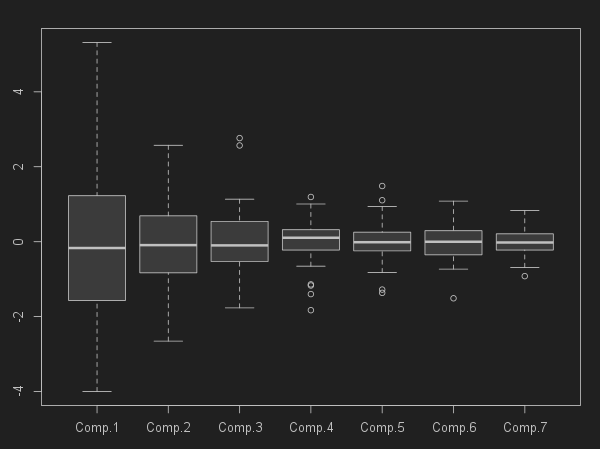
\includegraphics[width=0.5\linewidth]{img/bowplotcrimeacpscore}
        \caption{BoxPlot des données de robbery}
    \end{figure}

    \begin{figure}[H]
        \centering
        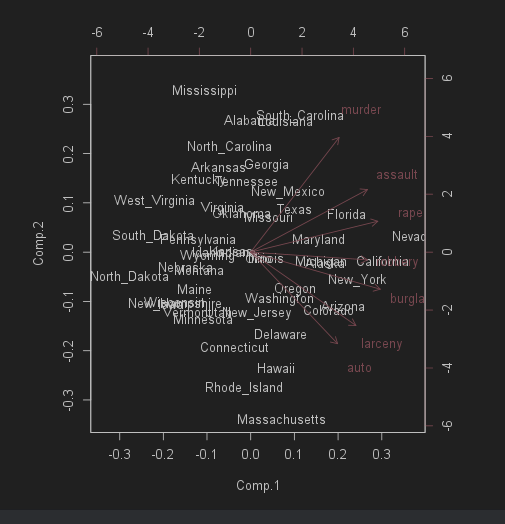
\includegraphics[width=0.5\linewidth]{img/bigplotcrimeacp}
        \caption{BoxPlot des données de robbery}
    \end{figure}

    \begin{figure}[H]
        \centering
        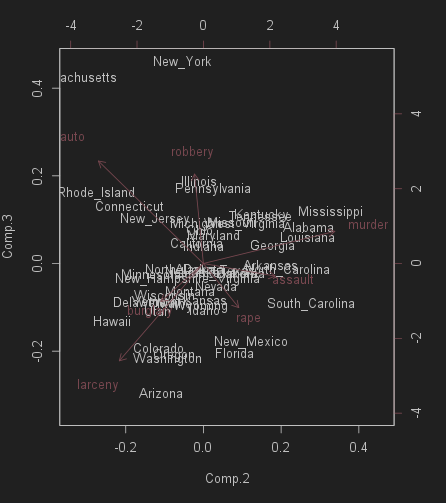
\includegraphics[width=0.5\linewidth]{img/bigplotcrimeacp2}
        \caption{BoxPlot des données de robbery}
    \end{figure}
    \textbf{Conclusion :} Les composantes 1et 2 suffisent pour bien représenter les données. La troisième n'apporte pas d’information significative supplémentaire.
    \subsubsection{Identification des valeurs atypiques sur la troisième composante}

    D’après l’ACP, deux états apparaissent comme \textbf{atypiques} sur la troisième composante : \textbf{New York} et \textbf{Massachusetts}.

    Ces valeurs influencent potentiellement la définition des axes. Il est recommandé de vérifier si leur exclusion modifie l’interprétation des résultats.

    \subsubsection{Exclusion des valeurs atypiques}

    Après avoir exclu \textbf{New York} et \textbf{Massachusetts}, vici les nouveaux biplots :

    \begin{figure}[H]
        \centering
        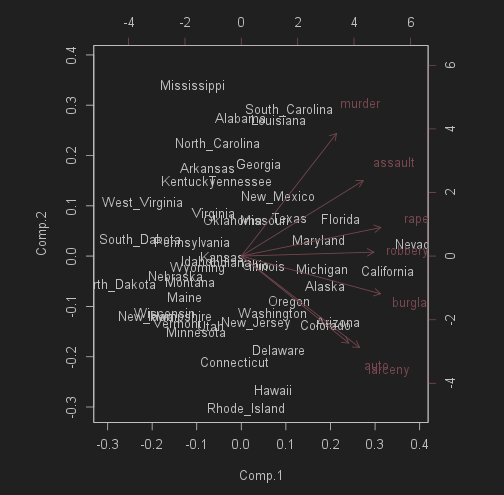
\includegraphics[width=0.5\linewidth]{img/bigplotcrimeacp3}
        \caption{Biplot des composantes 1 et 2 après exclusion}
    \end{figure}

    \begin{figure}[H]
        \centering
        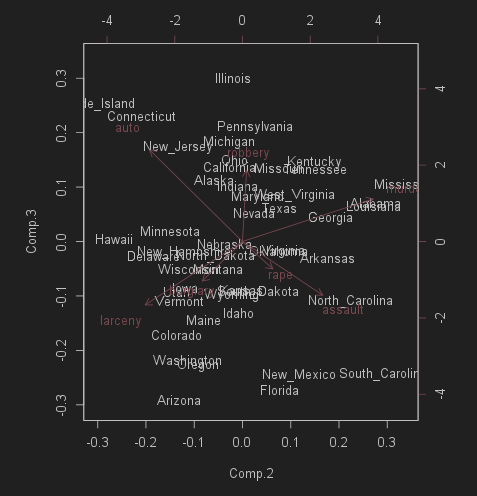
\includegraphics[width=0.6\linewidth]{img/bigplotcrimeacp4}
        \caption{Biplot des composantes 2 et 3 après exclusion}
    \end{figure}

    \textbf{Observations :}
    \begin{itemize}
        \item Le plan (\textbf{Comp.1, Comp.2}) reste similaire après l’exclusion.
        \item L’axe \textbf{Comp.3} est légèrement modifié,ce qui montre que ces états avaient une influence sur cette dimension.
    \end{itemize}

    \textbf{Conclusion :} L’exclusion n’affecte pas l’analyse globale mais réduit l’effet des valeurs extrêmes.

    \subsubsection{Interprétation des axes}
    je ne comprends pas cette question


    \section{Hôtels Méditerranéens}

    \subsection{ACP avec une variable qualitative supplémentaire}

    \subsubsection{Chargement des données}

    \subsubsection{Analyse des variables}

    Le jeu de données \texttt{hotels} contient 39 hôtels et 8 variables :

    \begin{itemize}
        \item \textbf{PAYS} : Variable qualitative indiquant le pays dimplantation (variable supplémentaire dans l'ACP).
        \item \textbf{ETOILE} : Nombre d’étoiles de l’hôtel (quantitative discrète).
        \item \textbf{CONFORT} : Niveau de confort noté sur une échelle (quantitative discrète).
        \item \textbf{CHAMBRE} : Nombre total de chambres (quantitative continue).
        \item \textbf{CUISINE} : Niveau d’équipement de la cuisine (quantitative discrète).
        \item \textbf{SPORT} : Niveau d’équipement sortif (quantitative discrète).
        \item \textbf{PLAGE} : Indicateur d’accès à une plage (quantitative discrète).
        \item \textbf{PRIX} : Prix moyen des chambres (quantitative continue).
    \end{itemize}

    \textbf{Individus analysés :} Chaque ligne du tableau correspond à un hôtel.

    \textbf{Statistiques descriptives :}

    \begin{figure}[H]
        \centering
        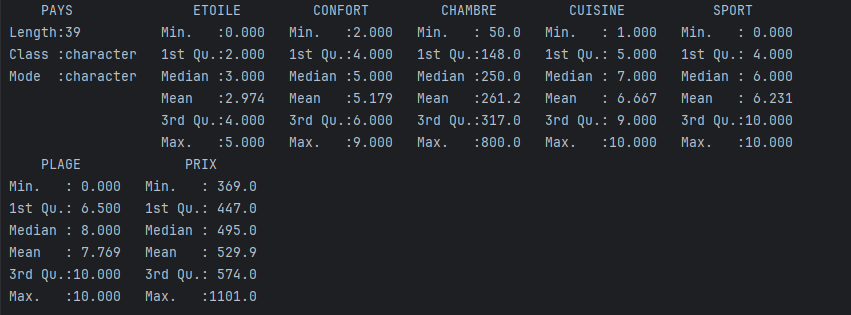
\includegraphics[width=0.6\linewidth]{img/summaryhotel}
        \caption{Biplot des composantes 2 et 3 après exclusion}
    \end{figure}

    \textbf{Covariances et corrélations :}

    \begin{figure}[H]
        \centering
        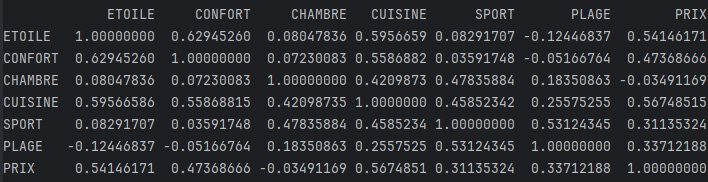
\includegraphics[width=0.6\linewidth]{img/covhotel}
        \caption{Biplot des composantes 2 et 3 après exclusion}
    \end{figure}

    On observe :
    \begin{itemize}
        \item Une \textbf{forte corrélation linéaire} entre \textbf{ÉTOILE et CONFORT} ($r = 0.63$).
        \item Une \textbf{corrélation notable} entre \textbf{ÉTOILE et CUISINE} ($r = 0.60$).
        \item Une \textbf{corrlation moyenne} entre \textbf{ÉTOILE et PRI} ($r = 0.54$), ce qui est attendu puisque les hôtels plus étoilés sont souvent plus chers.
        \item Peu de corrélations fortes entre les autres variables.
    \end{itemize}

    \textbf{Identification des liaisons non linéaires :}
    Si certaines relations ne sont pas linéaires, elles peuvent être visualisées avec :

    \begin{verbatim}
    pairs(hotels[,sapply(hotels, is.numeric)])
    \end{verbatim}

    \begin{figure}[H]
        \centering
        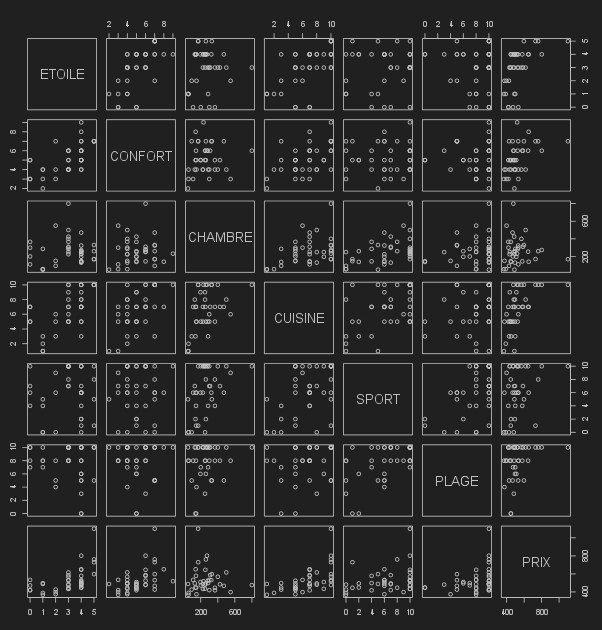
\includegraphics[width=0.6\linewidth]{img/pairhotel}
        \caption{Biplot des composantes 2 et 3 après exclusion}
    \end{figure}


    On observe des structures non linéaires, notamment entre :
    \begin{itemize}
        \item \textbf{PRIX et CUISINE}
        \item \textbf{SPORT et d'autres vaiables}
        \item \textbf{PLAGE et PRIX}
    \end{itemize}

    \subsubsection{Analyse en Composantes Principales}

    Les diagrammes des valeurs propres montrent l’inertie expliquée par chaque composante :

    \begin{figure}[H]
        \centering
        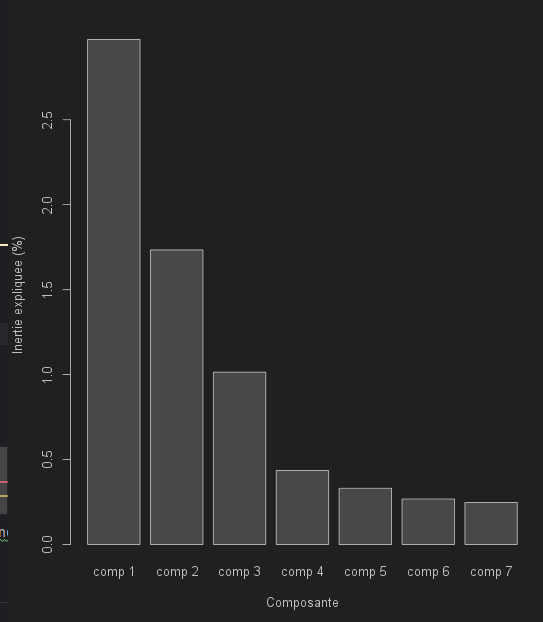
\includegraphics[width=0.6\linewidth]{img/inertie_expliquee}
        \caption{Inertie expliquée par composante}
    \end{figure}

    \begin{figure}[H]
        \centering
        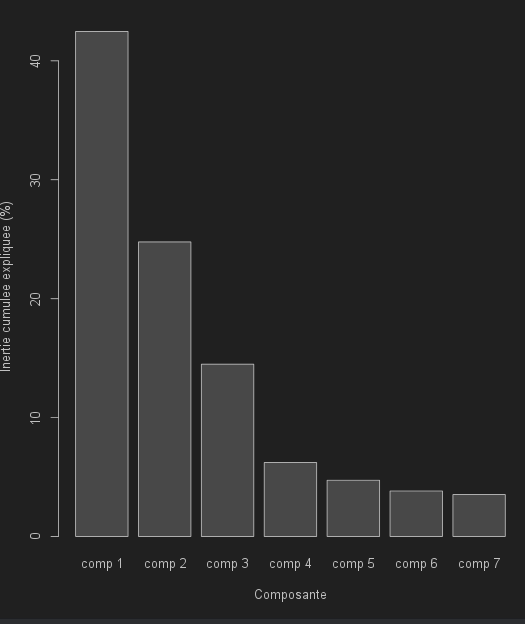
\includegraphics[width=0.6\linewidth]{img/inertie_cumulee}
        \caption{Inertie cumulée expliquée}
    \end{figure}

    L’inertie cumulée dépasse **40\% après la troisième cmposante** mais reste loin du seuil de **80\%**.
    Le choix optimal dépend du compromis entre simplification et information retenue, mais **3 composantes principales semblent suffisantes pour un bon résumé des données**.

    \subsubsection{Représentation des individus et des variables}

    Les individus (hôtels) sont représentés sur les premiers axes factoriels :

    \begin{figure}[H]
        \centering
        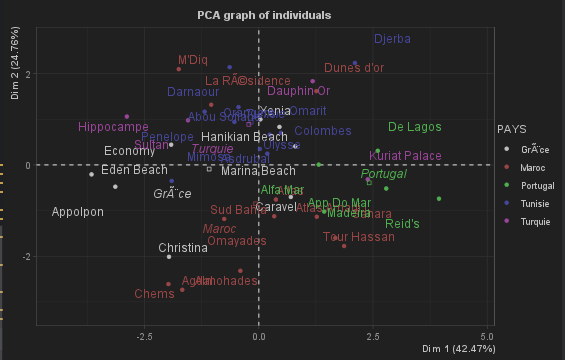
\includegraphics[width=0.6\linewidth]{img/PCA1.}
        \caption{Projection des individus sur Dim 1 et Dim 2}
    \end{figure}

    \begin{figure}[H]
        \centering
        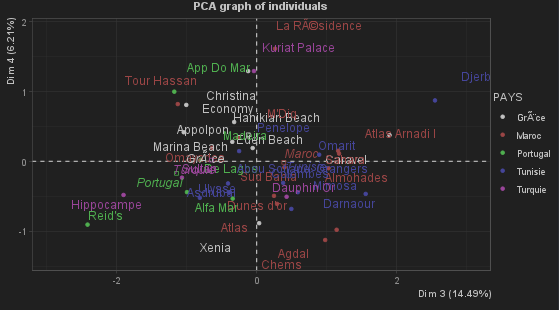
\includegraphics[width=0.6\linewidth]{img/PCA2}
        \caption{Projection des individus sur Dim 3 et Dim 4}
    \end{figure}

    Les variables sont représentées dans les cercles de corrélation :

    \begin{figure}[H]
        \centering
        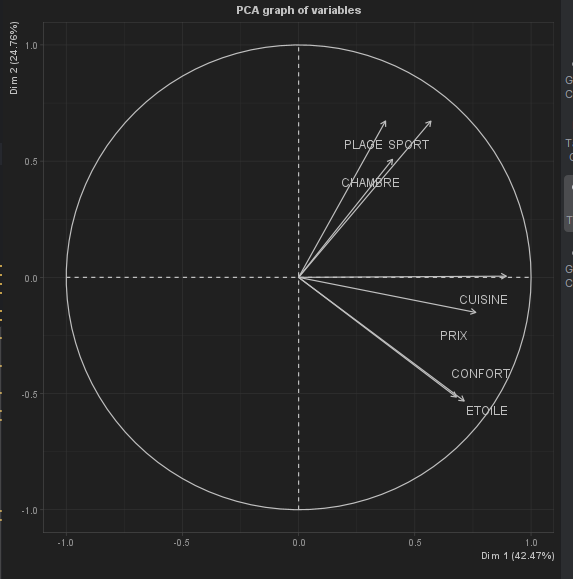
\includegraphics[width=0.6\linewidth]{img/PCA4}
        \caption{Cercle des corrélations - Dim 1 et Dim 2}
    \end{figure}

    \begin{figure}[H]
        \centering
        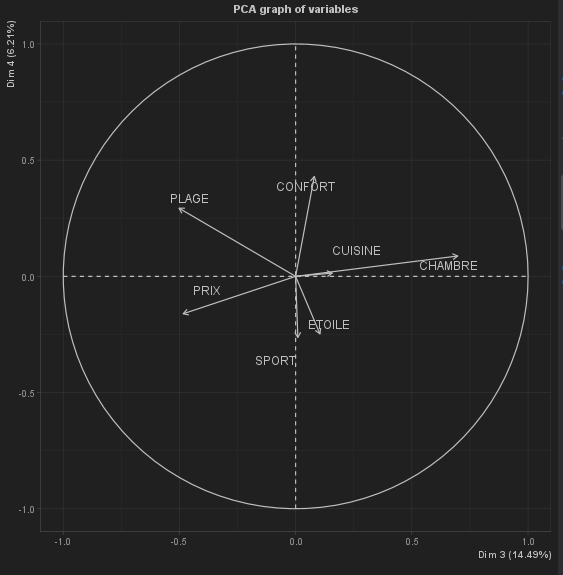
\includegraphics[width=0.6\linewidth]{img/PCA3}
        \caption{Cercle des corrélations - Dim 3 et Dim 4}
    \end{figure}

    L’analyse des représentations montre une bonne séparation des hôtels par pays sur les premiers axes et une forte structuration des variables dans les cercles de corrélation.

    \subsubsection{Utilisation de dimdesc}

    \begin{itemize}
        \item \textbf{Dimension 1} :
        \begin{itemize}
            \item Les variables continues les plus corréles sont \textbf{CUISINE} (0.89), \textbf{PRIX} (0.76) et \textbf{ETOILE} (0.71).
            \item La variable catégorielle \textbf{PAYS} est significative (\textit{p-value} = 0.006).
            \item Les pays \textbf{Portugal} et \textbf{Grèce} inluencent cette dimension.
        \end{itemize}

        \item \textbf{Dimension 2} :
        \begin{itemize}
            \item Les variables continues les plus corrélées sont \textbf{PLAGE} (0.67) et \textbf{SPORT} (0.67).
            \item La variable \textbf{PAYS} est aussi significative (\textit{p-value} = 0.009).
            \item Les pays \textbf{Tunisie} et \textbf{Maroc} influencent cette dimension.
        \end{itemize}

        \item \textbf{Dimension 3} :
        \begin{itemize}
            \item Les variables coninues les plus corrélées sont \textbf{CHAMBRE} (0.69) et \textbf{PRIX} (-0.48).
            \item La variable \textbf{PAYSl} est également significative (\textit{p-value} = 0.011).
            \item Le pays \textbf{Portugal} influence cette dimension.
        \end{itemize}
    \end{itemize}

    \subsubsection{Utilisation de coord.ellipse}
    \begin{figure}[H]
        \centering
        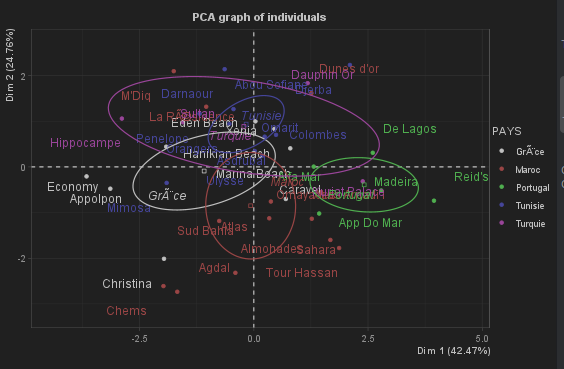
\includegraphics[width=0.6\linewidth]{img/PlotPCA1}
        \caption{Cercle des corrélations - Dim 3 et Dim 4}
    \end{figure}
    \begin{figure}[H]
        \centering
        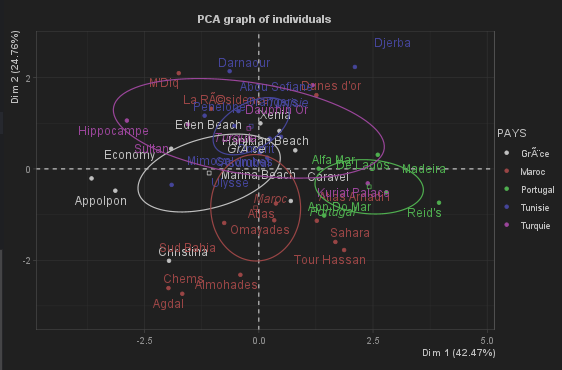
\includegraphics[width=0.6\linewidth]{img/PlotPCA2}
        \caption{Cercle des corrélations - Dim 3 et Dim 4}
    \end{figure}
    On observe que :
    \begin{itemize}
        \item Les hôtels situés au \textbf{Portugal} et au \textbf{Maroc} sont plutot bien distincts des autres groupes.
        \item La \textbf{Tnisie} et la \textbf{Turquie} présentent une forte superposition, suggérant que leurs hôtels partagent des caractéristiques similaires.
    \end{itemize}
    \subsection{ACP avec variables qualitative et quantitative supplémentaires}
    Ayant un projet a rendre pour lundi 10 février pour mon universitée eramsus en Italie, je n'ai pu commencer a travailler sur ce projet qu'aujourd'hui, je n'ai donc pas eu le temps de faire cette partie du TP.

\end{document}
